%!TEX root = lec16.tex
% ================================================================================
% Lecture 16, Slide 10
% ================================================================================
\begin{frame}[t]
  \mytitle{Step 2: Attention --- How the Model Understands Context}

\begin{columns}[T,totalwidth=\textwidth]

% ------------------------------------------------------------
\begin{column}[T]{0.50\textwidth}
\footnotesize
\vspace{3mm}

\textbf{\textcolor{blue}{Attention is selective reading}}

\vspace{2mm}
\begin{itemize}
  \item for each word, the model decides:
  \textbf{what earlier words matter}
  \item it forms weighted links between tokens
  \item repeated many times in layers
\end{itemize}

\vspace{4mm}
\textbf{\textcolor{red}{Key point:}}
\quad Attention allows \y{long-range dependencies}
and structured reasoning.

\end{column}

% ------------------------------------------------------------
\begin{column}[T]{0.46\textwidth}
\footnotesize
\vspace{3mm}

\textbf{\textcolor{violet}{A simple intuition}}

\vspace{2mm}
\begin{itemize}
  \item Like humans:
  \textbf{scan} + \textbf{focus} + \textbf{connect}
  \item Not one focus, but many:
  {\tiny \newline (\textbf{multi-head attention})}
\end{itemize}

\vspace{3mm}
{\tiny \textcolor{gray}{
Transformer = many attention layers + feed-forward layers.
}}
\end{column}

\end{columns}

% ------------------------------------------------------------
% Attention diagram (TikZ)
% ------------------------------------------------------------
\vspace{2mm}

\vspace{-1.5cm}
\hspace*{5cm}\scalebox{0.85}{
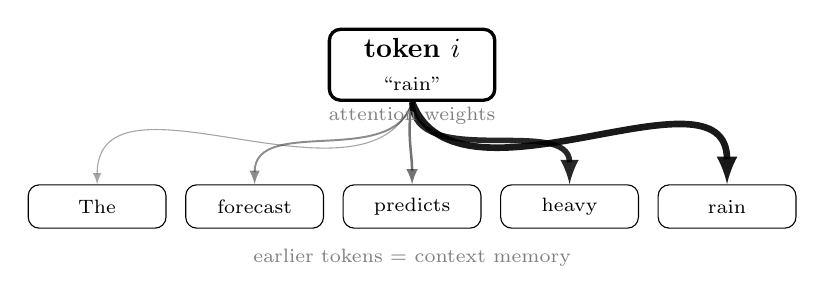
\begin{tikzpicture}[>=latex, x=1cm, y=1cm]

\tikzstyle{tok}=[draw, rounded corners, minimum width=1.75cm, minimum height=0.55cm, align=center]
\tikzstyle{qtok}=[draw, rounded corners, minimum width=2.1cm, minimum height=0.60cm, align=center, very thick]

% --- top: current token (query) ---
\node[qtok] (q) at (0,1.8) {\textbf{token $i$}\\{\scriptsize ``rain''}};

% --- bottom: context tokens (keys/values) ---
\node[tok] (t1) at (-4.0,0) {\scriptsize The};
\node[tok] (t2) at (-2.0,0) {\scriptsize forecast};
\node[tok] (t3) at ( 0.0,0) {\scriptsize predicts};
\node[tok] (t4) at ( 2.0,0) {\scriptsize heavy};
\node[tok] (t5) at ( 4.0,0) {\scriptsize rain};

% --- arrows = attention weights ---
\draw[->, line width=0.4pt, opacity=0.35] (q.south) to[out=250,in=90] (t1.north);
\draw[->, line width=0.7pt, opacity=0.45] (q.south) to[out=255,in=90] (t2.north);
\draw[->, line width=0.9pt, opacity=0.55] (q.south) to[out=260,in=90] (t3.north);
\draw[->, line width=2.0pt, opacity=0.85] (q.south) to[out=270,in=90] (t4.north);
\draw[->, line width=2.4pt, opacity=0.90] (q.south) to[out=290,in=90] (t5.north);

% --- labels ---
\node[align=center] at (0,1.15) {\scriptsize \textcolor{gray}{attention weights}};
\node[align=center] at (0,-0.65) {\scriptsize \textcolor{gray}{earlier tokens = context memory}};

\end{tikzpicture}
}

\end{frame}
